\documentclass[12pt]{exam}
\usepackage[margin=1in]{geometry}
\usepackage{graphicx}
\usepackage{amsmath}
\usepackage{amssymb}
\usepackage{xcolor}
\usepackage{xeCJK}
\usepackage{tikz}
\setCJKmainfont{KaiTi}

\header{循人中学}{2017年第二学期期末考}{高一数学}
\footer{}{- \;\thepage \; -}{} 

\printanswers
\shadedsolutions
%\pointsinrightmargin
\renewcommand{\solutiontitle}{\noindent}
\renewcommand{\ge}{\geqslant}
\renewcommand{\geq}{\geqslant}
\renewcommand{\le}{\leqslant}
\renewcommand{\leq}{\leqslant}
\definecolor{SolutionColor}{rgb}{1.0,0.98,0.8}

\begin{document}
\begin{titlepage}
\begin{center}

\vspace*{1cm}

{\Huge 循人中学}\\[0.5cm]
{\Large TSUN JIN HIGH SCHOOL}\\[1cm]
\noindent\rule{12cm}{1.5pt}\\[0.6cm]
{\huge 2017年第二学期期末考}\\[0.3cm]
{\Large 高一数学}\\[0.3cm]

\noindent\rule{12cm}{1.5pt}\\[1cm]

\begin{tikzpicture}
\node[draw, rectangle, rounded corners=10pt, line width=2pt, 
      minimum width=13cm, minimum height=3cm, align=center] {
      {\LARGE 《高一备考数学题精选集之:}\\[0.4cm]
      {\LARGE 一题都别想做》}
};
\end{tikzpicture}

\vspace{1cm}

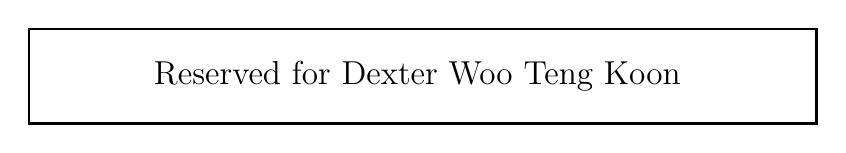
\begin{tikzpicture}
\node[draw, rectangle, line width=1pt, 
      minimum width=10cm, minimum height=1.2cm, align=center] {
      \large Reserved for Dexter Woo Teng Koon
};
\end{tikzpicture}

\vspace{1cm}

\begin{tabular}{|p{4cm}|p{4cm}|}
\hline
\rule{0pt}{1cm}A、必答题 & 90分\\[0.5cm]
\hline
\rule{0pt}{1cm}B、选答题 & 10分(2选1) \\[0.5cm]
\hline
\rule{0pt}{1cm}总分 & 100分 \\[0.5cm]
\hline
\end{tabular}

\vspace{1cm}

{\large \textit{由于题量太大,作答时间为24小时,作答愉快!}}

\vspace{0.5cm}

\end{center}
\end{titlepage}
\newpage

\vspace{0.5cm}
\section*{A、必答题 (90\%)}

\begin{questions}
\question 
\begin{parts}
\part 若$\theta$为锐角,试证 
\[
\tan\frac{\theta}{2} = \sqrt{\frac{1 - \cos\theta}{1 + \cos\theta}}
\] 
据此, 试证 
\[
\tan\theta + \tan\frac{\theta}{2} = \csc\theta - 2\cot 2\theta
\]
\hfill (4分)
\begin{solution}
    由恒等式
    \[
    \sin^2\frac{\theta}{2} = \frac{1-\cos\theta}{2}, \quad \cos^2\frac{\theta}{2} = \frac{1+\cos\theta}{2}
    \]
    有
    \[
    \tan^2\frac{\theta}{2} = \frac{\sin^2\frac{\theta}{2}}{\cos^2\frac{\theta}{2}} = \frac{1-\cos\theta}{1+\cos\theta}
    \]
    由于$\theta$为锐角,于是
    \[
    \tan\frac{\theta}{2} = \sqrt{\frac{1-\cos\theta}{1+\cos\theta}}>0
    \]
    且有
    \begin{align*}
    \tan \theta + \tan \frac{\theta}{2} &= \frac{\sin \theta}{\cos \theta} + \sqrt{\frac{1 - \cos \theta}{1 + \cos \theta}} \\
    &= \frac{\sin \theta}{\cos \theta} + \sqrt{\frac{(1 - \cos \theta)^2}{1 - \cos^2 \theta}} \\
    &= \frac{\sin \theta}{\cos \theta} + \frac{1 - \cos \theta}{\sin \theta} \\
    &= \frac{\cos \theta - (\cos^2 \theta - \sin^2 \theta)}{\sin \theta \cos \theta} \\
    &= \frac{1}{\sin \theta} - \frac{2 \cos 2\theta}{2 \sin \theta \cos \theta} \\
    &= \frac{1}{\sin \theta} - \frac{2 \cos 2\theta}{\sin 2\theta} \\
    &= \csc \theta - 2 \cot 2\theta
    \end{align*}
\end{solution}

\part 已知 $\sin\theta + \sec\theta = \cos\theta + \csc\theta$, 求证: 
\[
\cos 2\theta + 4\cot 2\theta \csc 2\theta = 2(\tan\theta - \cot\theta)
\]
\hfill (4分)
\begin{solution}
    \begin{align*}
    \cos 2\theta + 4 \cot 2\theta \csc 2\theta 
    &= \cos^2\theta - \sin^2\theta +\frac{4\cos 2\theta}{\sin^2 2\theta} \\
    &= \cos^2\theta - \sin^2\theta + \frac{\cos^2\theta - \sin^2\theta}{\sin^2\theta \cos^2\theta} \\
    &= \cos^2\theta - \sin^2\theta + \csc^2\theta - \sec^2\theta \\
    &= (\cos\theta + \csc\theta)^2 - 2 \cot\theta - (\sin\theta + \sec\theta)^2 + 2 \tan\theta \\
    &= 2 (\tan\theta - \cot\theta)
    \end{align*}
    故得证。
\end{solution}
\end{parts}

\question 
\begin{parts}
\part 解 
\[
(\cos^{2}\theta - 1)(\sin^{2}\theta - 1) < 0, 
\]
式中 $-2\pi \leq \theta \leq 2\pi$。\hfill (2分)
\begin{solution}
    注意到
    \[
    \cos^2\theta - 1 = -\sin^2\theta, \quad \sin^2\theta - 1 = -\cos^2\theta
    \]
    因此
    \[
    (\cos^2\theta - 1)(\sin^2\theta - 1) = (-\sin^2\theta)(-\cos^2\theta) = \sin^2\theta\cos^2\theta \geq 0
    \]
    于是原不等式无解。
\end{solution}

\part 解三角方程式 
\[
16\sin^{2}\theta + \tan^{2}\theta + 9(\csc^{2}\theta + \cot^{2}\theta) = 30, 
\]
其中 $0^\circ \leq \theta \leq 360^\circ$。\hfill (5分)
\begin{solution}
    原方程式即
    \[
    (4 \sin\theta - 3 \csc\theta)^2 + (\tan\theta - 3 \cot\theta)^2 = 0
    \]
    于是
    \[
    4 \sin\theta - 3 \csc\theta = 0 \Rightarrow \sin\theta = \pm\frac{\sqrt{3}}{2} \Rightarrow \theta =60^\circ, 120^\circ, 240^\circ, 300^\circ
    \]
    且
    \[
    \tan\theta - 3 \cot\theta = 0 \Rightarrow \tan\theta = \pm\sqrt{3} \Rightarrow \theta = 60^\circ, 120^\circ, 240^\circ, 300^\circ
    \]
    故原方程式的解为
    \[
    \theta = 60^\circ, 120^\circ, 240^\circ, 300^\circ
    \]
\end{solution}

\part 解 
\[
\sin^{8}\theta + \cos^{8}\theta = \frac{17}{32},
\] 
式中 $0^\circ \leq \theta \leq 360^\circ$。\hfill (5分)
\begin{solution}
    化简得
    \begin{align*}
    \sin^8 \theta + \cos^8 \theta &= \frac{17}{32} \\
    (\sin^4 \theta + \cos^4 \theta)^2 - 2 \sin^4 \theta \cos^4 \theta &= \frac{17}{32} \\
    \left((\sin^2 \theta + \cos^2 \theta)^2 - 2 \sin^2 \theta \cos^2 \theta\right)^2 - 2 \sin^4 \theta \cos^4 \theta &= \frac{17}{32} \\
    (1 - 2 \sin^2 \theta \cos^2 \theta)^2 - 2 \sin^4 \theta \cos^4 \theta &= \frac{17}{32} \\
    2 \sin^4 \theta \cos^4 \theta - 4 \sin^2 \theta \cos^2 \theta + \frac{15}{32} &= 0 \\
    4 \sin^2 2\theta - 32 \sin^2 2\theta + 15 &= 0 \\
    (2 \sin^2 2\theta - 1)(2 \sin^2 2\theta - 15) &= 0
    \end{align*}
    于是由$\sin^2 2\theta = \dfrac{1}{2} \Rightarrow \sin 2\theta = \pm \dfrac{\sqrt{2}}{2}$,解为
    \begin{align*}
        2\theta &= 45^\circ, 135^\circ, 225^\circ, 315^\circ, 405^\circ, 495^\circ, 585^\circ, 675^\circ \\
        \theta &= 22.5^\circ, 67.5^\circ, 112.5^\circ, 157.5^\circ, 202.5^\circ, 247.5^\circ, 292.5^\circ, 337.5^\circ
    \end{align*}
    其中由于$0 \leq \sin^2 \alpha \leq 1, \alpha \in \mathbb{R}$,方程式$\sin^2 2\theta = \dfrac{15}{2}$无解。
\end{solution}
\end{parts}

\question 
\begin{parts}
\part 若 $\alpha = \dfrac{2\pi}{1999}$, 试求 
\[
\cos\alpha\cos 2\alpha\cos 3\alpha\ldots\cos 998\alpha\cos 999\alpha
\]
的值。
\hfill (6分)
\begin{solution}
    记$S = \cos \alpha \cos 2\alpha \cdots \cos 999\alpha, T = \sin \alpha \sin 2\alpha \cdots \sin 999\alpha$,则
    \[
    ST = \sin \alpha \cos \alpha \sin 2\alpha \cos 2\alpha \cdots \sin 999\alpha \cos 999\alpha 
    \]
    即
    \[
    2^{999} ST = \sin 2\alpha \sin 4\alpha \cdots \sin 1998\alpha
    \]
    且注意到
    \[
    \sin 1998\alpha = - \sin(2\pi - 1998\alpha) = - \sin\frac{2\pi}{1999} = - \sin \alpha
    \]
    同理,
    \[
    \sin 1996\alpha = - \sin 3\alpha, \quad \sin 1994\alpha = - \sin 5\alpha, \cdots
    \]
    因此
    \[
    2^{999} ST = \sin \alpha \sin 4\alpha \cdots (-\sin 3\alpha)(-\sin \alpha) = \sin \alpha \sin 4\alpha \cdots \sin 3\alpha \sin \alpha = T 
    \]
    由于 $T \neq 0$,故
    \[
    S = \cos \alpha \cos 2\alpha \cos 3\alpha \cdots \cos 998\alpha \cos 999\alpha = \frac{1}{2^{999}}
    \]
\end{solution}

\part 证对于任意角 $A,B,C$, 均有
\[
\sin A + \sin B + \sin C - \sin(A + B + C) = 4\sin\frac{A+B}{2}\sin\frac{B+C}{2}\sin\frac{C+A}{2}
\]
\hfill (6分)
\begin{solution}
    由和差化积公式,
    \begin{align*}
    &\sin A + \sin B + \sin C - \sin(A+B+C) \\
    &= 2\sin\frac{A+B}{2}\cos\frac{A-B}{2} + \sin C - (\sin(A+B)\cos C + \cos(A+B)\sin C) \\
    &= 2\sin\frac{A+B}{2}\cos\frac{A-B}{2} - 2\sin\frac{A+B}{2}\cos\frac{A+B}{2}\cos C + \sin C(1-\cos(A+B)) \\
    &= 2\sin\frac{A+B}{2}\left(\cos\frac{A-B}{2} - \cos\frac{A+B}{2}\cos C\right) + \sin C\left(2\sin^2\frac{A+B}{2}\right) \\
    &= 2\sin\frac{A+B}{2}\left[\cos\frac{A-B}{2} - \left(\cos\frac{A+B}{2}\cos\frac{C}{2} - \sin\frac{A+B}{2}\sin\frac{C}{2}\right)\right] \\
    &= 2\sin\frac{A+B}{2}\left[\cos\left(\frac{A+C}{2}-\frac{B+C}{2}\right) - \cos\left(\frac{C+A}{2}+\frac{B+C}{2}\right)\right] \\
    &= 4\sin\frac{A+B}{2}\sin\frac{B+C}{2}\sin\frac{C+A}{2}
    \end{align*}
\end{solution}
\end{parts}

\question 
\begin{parts}
\part 解方程式 
\[
\log_{x}x + \log_{x}3 = 1
\]
\hfill (2分)
\begin{solution}
    由原方程,
    \[
    1 + \log_x 3 = 1 \Rightarrow \log_x 3 = 0
    \]
    此方程无解,故原方程式无解。
\end{solution}

\part 解 
\[
x^{x^{x}} = (x^{x})^{x}
\]
\hfill (4分)
\begin{solution}
    原方程即
    \[
    x^{x^{x}} = x^{x^2}
    \]
    先考虑指数方程的特殊情况$x=-1,0,1$,可得解
    \[
    x=-1,1
    \]
    当$x \neq -1,0,1$时,由底数相等所以指数相等的性质得,
    \[
    x=2
    \]
    故原方程式的解为
    \[
    x=-1 \quad \text{或} \quad x=1 \quad \text{或} \quad x=2
    \]
\end{solution}

\part 已知 
\[
\frac{\log a}{b - c} = \frac{\log b}{c - a} = \frac{\log c}{a - b},
\]
其中 $a \neq b \neq c$, 试求 $a^{a}b^{b}c^{c}$ 的值。\hfill (4分)
\begin{solution}
    设
    \[
    \frac{\log a}{b-c} = \frac{\log b}{c-a} = \frac{\log c}{a-b} = k
    \]
    则
    \[
    \log a = k(b-c), \quad \log b = k(c-a), \quad \log c = k(a-b)
    \]
    因此
    \begin{align*}
    \log(a^a b^b c^c) &= a\log a + b\log b + c\log c \\
    &= ak(b-c) + bk(c-a) + ck(a-b) \\
    &= k[ab - ac + bc - ab + ca - cb] \\
    &= 0
    \end{align*}
    即 
    \[
    a^a b^b c^c = 1
    \]
\end{solution}
\end{parts}

\question 
\begin{parts}
\part 若正实数 $x,y,z$ 满足
\[
\begin{cases}
\log_{2}x + \log_{4}y + \log_{4}z = 2 \\
\log_{3}y + \log_{9}z + \log_{9}x = 2 \\
\log_{4}z + \log_{16}x + \log_{16}y = 2
\end{cases}
\]
求 $xyz$。\hfill (4分)
\begin{solution}
    原方程组给出
    \[
    \begin{cases}
    \log_2 x + \log_2 \sqrt{y} + \log_2 \sqrt{z} = 2 \Rightarrow x\sqrt{yz} = 2^2 \\
    \log_3 y + \log_3 \sqrt{z} + \log_3 \sqrt{x} = 2 \Rightarrow y\sqrt{xz} = 3^2 \\
    \log_4 z + \log_4 \sqrt{x} + \log_4 \sqrt{y} = 2
    \Rightarrow z\sqrt{xy} = 4^2
    \end{cases}
    \]
    将三式相乘得
    \[
    (xyz)^2 = 2^6 \cdot 3^2 \Rightarrow xyz = 24 > 0
    \]
\end{solution}

\part 解方程式 
\[
(\log_{5}x)^{2} + \log_{5x}\left(\frac{5}{x}\right) = 1
\]
\hfill (4分)
\begin{solution}
    设$\log_5 x = t$,则
    \[
    \log_{5x}\left(\frac{5}{x}\right) = \frac{\log_5\frac{5}{x}}{\log_5(5x)} = \frac{\log_5 5 - \log_5 x}{\log_5 5 + \log_5 x} = \frac{1-t}{1+t}
    \]
    原方程式变为
    \begin{align*}
    t^2 + \frac{1-t}{1+t} &= 1 \\
    t^2(1+t) + 1-t &= 1+t \\
    t^3 + t^2 - 2t &= 0 \\
    t(t+2)(t-1) &= 0
    \end{align*}
    解得 $t = 0, -2, 1$,即 
    \[
    x = 5^0 = 1, \quad \text{或} \quad x = 5^{-2} = \frac{1}{25}, \quad \text{或} \quad x = 5^1 = 5
    \]
    经检验得$x = 1, x = \dfrac{1}{25}, x=5$都是原方程的解。
\end{solution}

\part 已知 
\[
(x\sqrt{x}\sqrt[3]{x})^{x} = x^{x\sqrt{x}\sqrt[3]{x}},
\]
试求 $x^{5}$ 的值。\hfill (5分)
\begin{solution}
    \begin{align*}
    (x\sqrt{x}\sqrt[3]{x})^{x} &= x^{x\sqrt{x}\sqrt[3]{x}} \\
    x^{(1+\frac{1}{2}+\frac{1}{3})x} &= x^{x^{1+\frac{1}{2}+\frac{1}{3}}}\\
    x^{(\frac{11}{6})x} &= x^{x^{\frac{11}{6}}}
    \end{align*}
    考虑特殊情况 $x=-1, 0, 1,$ 可得解 $x=1$。若$x \neq -1, 0, 1,$因底数相等所以指数相等,得
    \[
    \frac{11}{6}x = x^{\frac{11}{6}} \Rightarrow x^5 = \left(\frac{11}{6}\right)^{6} 
    \]
    故$x^5$的可能值为
    \[
    x^5=1 \quad \text{或} \quad x^5 = \left(\frac{11}{6}\right)^{6}
    \]
\end{solution}
\end{parts}

\question 
\begin{parts}
\part 已知正实数 $a,b$ 满足 $a + b = 1$,求 
\begin{subparts}
\subpart $ab^{2017}$ 的最大值; \hfill (4分)
\begin{solution}
    由AM-GM不等式,
    \[
    \frac{1}{2018}=\frac{a+\underbrace{\frac{b}{2017}+\dots+\frac{b}{2017}}_{2017's}}{2018} \ge \sqrt[2018]{\frac{ab^{2017}}{2017^{2017}}}
    \]
    即
    \[
    ab^{2017} \le \frac{2017^{2017}}{2018^{2018}}
    \]
    当 $a = \dfrac{1}{2018}, b = \dfrac{2017}{2018}$时等号成立,此时 $ab^{2017}$ 有最大值 $\dfrac{2017^{2017}}{2018^{2018}}$
\end{solution}
\subpart $\left(a + \dfrac{1}{a}\right)^{2} + \left(b + \dfrac{1}{b}\right)^{2}$ 的最小值。\hfill (4分)
\begin{solution}
    由柯西不等式或QM-AM不等式, 
    \[
    \left(a+\frac{1}{a}\right)^2+\left(b+\frac{1}{b}\right)^2
    \ge
    \frac12\left(a+b+\frac{1}{a}+\frac{1}{b}\right)^2=\frac12\left(1+\frac{1}{ab}\right)^2
    \]
    又由AM-GM不等式,
    \[
    ab\le\left(\frac{a+b}{2}\right)^2=\frac14
    \]
    故
    \[
    \left(a+\frac{1}{a}\right)^2+\left(b+\frac{1}{b}\right)^2
    \ge
    \frac12\cdot (1+4)^2=\frac{25}{2}
    \]
    当且仅当 $a=b=\dfrac12$ 时等号成立,此时有最小值 $\dfrac{25}{2}$。
\end{solution}
\end{subparts}
\part 已知实数$a,b,c,d$满足 
\[
ab + bc + cd = 8,\quad b^{2} + c^{2} = 2,
\]
试求 $a^{2} + d^{2}$ 的最小值。\hfill (5分)
\begin{solution}
    首先有
    \[
    b^2+c^2 \ge 2bc \Rightarrow bc \le 1
    \]
    由柯西不等式,
    \[ 
    (a^2+d^2)(b^2+c^2) \ge (ab+cd)^2 
    \]
    即
    \[ 
    (a^2+d^2) \ge \frac{(ab+cd)^2}{b^2+c^2} = \frac{(8-bc)^2}{2} \ge \frac{(8-1)^2}{2} = \frac{49}{2} 
    \]
    当 $b=c$ 且 $\dfrac{a}{c} = \dfrac{d}{b}$, 即 $b=c=-1,a=d=-\dfrac{7}{2}$ 时等号成立,此时$a^2+d^2$ 取最小值 $\dfrac{49}{2}$。
\end{solution}

\part 已知实数$a,b,c$满足 $a^{2} + b^{2} + c^{2} = 1$, 求 
\[
\left(\frac{1}{1 + 2ab - c^{2}} + \frac{1}{1 + 2bc - a^{2}} + \frac{1}{1 + 2ca - b^{2}}\right)^{2}
\]
的最小值。\hfill (5分)
\begin{solution}
    由柯西不等式,
    \begin{align*}
    &\frac{1^2}{1+2ab-c^2} + \frac{1^2}{1+2bc-a^2} + \frac{1^2}{1+2ca-b^2} \\
    &\ge \frac{(1+1+1)^2}{(1+2ab-c^2)+(1+2bc-a^2)+(1+2ca-b^2)} \\
    &= \frac{9}{2+2(ab+bc+ca)}
    \end{align*}
    由排序不等式,
    \[
    1=a^{2} + b^{2} + c^{2} \ge ab + bc + ca
    \]
    于是
    \[
    \left(\frac{1}{1 + 2ab - c^{2}} + \frac{1}{1 + 2bc - a^{2}} + \frac{1}{1 + 2ca - b^{2}}\right)^{2} \ge \left(\frac{9}{2+2}\right)^{2} = \frac{81}{16}
    \]
    等号成立当且仅当 $a=b=c=\pm\dfrac{\sqrt{3}}{3}$。
\end{solution}
\end{parts}

\question 
\begin{parts}
\part 求 
\[
\sum_{r=1}^{\infty}\frac{1}{r(r + 1)(r + 2)(r + 3)}
\]
\hfill (4分)
\begin{solution}
利用部分分式分解得
\[
\frac{1}{r(r+1)(r+2)(r+3)} = \frac{1}{3}\left[\frac{1}{r(r+1)(r+2)} - \frac{1}{(r+1)(r+2)(r+3)}\right]
\]
因此原式是一裂项求和,有
\begin{align*}
\sum_{r=1}^{\infty}\frac{1}{r(r+1)(r+2)(r+3)} &= \frac{1}{3}\left[\frac{1}{1 \cdot 2 \cdot 3} - \lim_{n\to\infty}\frac{1}{(n+1)(n+2)(n+3)}\right] \\
&= \frac{1}{3} \cdot \frac{1}{6} - 0 \\
&= \frac{1}{18}
\end{align*}
\end{solution}

\part 已知 
\[ 
1 + \frac{1}{2^{2}} + \frac{1}{3^{2}} + \frac{1}{4^{2}} + \cdots = \frac{\pi^{2}}{6},
\]
试求 
\[
1 + \frac{1}{3^{2}} + \frac{1}{5^{2}} + \frac{1}{7^{2}} + \cdots
\]
的值。\hfill (4分)
\begin{solution}
    设
    \[
    S = 1 + \frac{1}{3^2} + \frac{1}{5^2} + \frac{1}{7^2} + \cdots
    \]
    则
    \[
    \frac{\pi^2}{6} = S + \left( \frac{1}{2^2} + \frac{1}{4^2} + \frac{1}{6^2} + \cdots \right) = S + \frac{1}{2^2}\left(1 + \frac{1}{2^2} + \frac{1}{3^2} + \cdots\right)= S + \frac{1}{4} \cdot \frac{\pi^2}{6}
    \]
    解得
    \[
    S = \frac{\pi^2}{8}
    \]
\end{solution}
\end{parts}

\question 
\begin{parts}
\part 试证 
\[
8 + 88 + 888 + \ldots + \underbrace{888\ldots88}_{\text{88's}} = \frac{8}{81}(10^{89} - 802)
\] 
\hfill (4分)
\begin{solution}
    考虑到
    \[
    \underbrace{99\ldots99}_{\text{n's}}= 10^n - 1
    \]
    于是
    \begin{align*}
    8 + 88 + 888 + \cdots + \underbrace{888\ldots88}_{\text{88's}} 
    &= \frac{8}{9}(9 + 99 + 999 + \cdots + \underbrace{99\ldots99}_{\text{88's}}) \\
    &= \frac{8}{9}(10 + 10^2 + 10^3 + \cdots + 10^{88} - 88) \\
    &= \frac{8}{9}\left[\frac{10(10^{88}-1)}{10-1}-88\right] \\
    &= \frac{8}{81}(10^{89} - 802)
    \end{align*}
    故得证。
\end{solution}

\part 求无穷级数
\[
\frac{1^{2}}{11} + \frac{5^{2}}{11^{2}} + \frac{9^{2}}{11^{3}} + \frac{13^{2}}{11^{4}} + \cdots + \frac{(4n - 3)^{2}}{11^{n}} + \cdots
\]
\hfill (5分)
\begin{solution}
    设原式为 
    \[
    S = \sum_{n=1}^{\infty}\frac{(4n-3)^2}{11^n}
    \]
    由 $(4n-3)^2 = 16n^2 - 24n + 9$,有
    \[
    S = 16\sum_{n=1}^{\infty}\frac{n^2}{11^n} - 24\sum_{n=1}^{\infty}\frac{n}{11^n} + 9\sum_{n=1}^{\infty}\frac{1}{11^n}
    \]
    当 $|x| < 1$ 时,有
    \[
    \sum_{n=1}^{\infty}x^n = \frac{x}{1-x}, \quad
    \sum_{n=1}^{\infty}nx^n = \frac{x}{(1-x)^2}, \quad
    \sum_{n=1}^{\infty}n^2x^n = \frac{x(1+x)}{(1-x)^3}
    \]
    令 $x = \dfrac{1}{11}$, 则
    \[
    \sum_{n=1}^{\infty}\frac{1}{11^n} = \frac{1}{10}, \quad \sum_{n=1}^{\infty}\frac{n}{11^n} = \frac{11}{100}, \quad \sum_{n=1}^{\infty}\frac{n^2}{11^n} = \frac{33}{250}
    \]
    于是
    \[
    S = 16 \cdot \frac{33}{250} - 24 \cdot \frac{11}{100} + 9 \cdot \frac{1}{10} = \frac{93}{250}
    \]
\end{solution}
\begin{solution}
    设
    \[
    S=\frac{1^{2}}{11} + \frac{5^{2}}{11^{2}} + \frac{9^{2}}{11^{3}} + \frac{13^{2}}{11^{4}} + \frac{17^{2}}{11^{5}} + \cdots \tag{1}
    \]
    则
    \[
    \frac{1}{11}S=\frac{1^{2}}{11^2} + \frac{5^{2}}{11^{3}} + \frac{9^{2}}{11^{4}} + \frac{13^{2}}{11^{5}} + \frac{17^{2}}{11^{6}} + \cdots \tag{2}
    \]
    (1) - (2) 得
    \[
    \frac{10}{11} S = \frac{1}{11} + \frac{5^2-1^2}{11^2} + \frac{9^2-5^2}{11^3} + \frac{13^2-9^2}{11^4} + \frac{17^2-13^2}{11^5} + \cdots \tag{3}
    \]
    \[
    \frac{10}{121} S = \frac{1}{11^2} + \frac{5^2-1^2}{11^3} + \frac{9^2-5^2}{11^4} + \frac{13^2-9^2}{11^5} + \frac{17^2-13^2}{11^6} + \cdots \tag{4}
    \]
    (3) - (4) 得
    \[
    \frac{100}{121} S = \frac{1}{11} + \frac{23}{11^2} + \frac{32}{11^3} + \frac{32}{11^4} + \frac{32}{11^5} + \cdots = \frac{1}{11} + \frac{23}{11^2} + \frac{32}{11^3} \cdot \frac{1}{1 - \frac{1}{11}}
    \]
    故可得
    \[
    S = \frac{93}{250}
    \]
\end{solution}
\end{parts}

\end{questions}

\newpage
\section*{B、选答题 (2选1) (10\%)}

\begin{questions}
\setcounter{question}{0}

\question 
\begin{parts}
\part 试证 
\[
2^{\sqrt{\log_{2}3}} = 3^{\sqrt{\log_{3}2}}
\]
\hfill (2分)
\begin{solution}
    注意到
    \[
    2^{\sqrt{\log_2 3}} 
    = 2^{\frac{\log_2 3}{\sqrt{\log_2 3}}} 
    = \left(2^{\log_2 3}\right)^{\sqrt{\log_3 2}} 
    = 3^{\sqrt{\log_3 2}}
    \]
    故左式等于右式,得证。
\end{solution}

\part 求 
\[
|x - 1|^{\log_{2}(4 - x)} < |x - 1|^{\log_{2}(1 + x)}
\]
的解之范围。
\hfill (4分)
\begin{solution}
    由$\log_{2}(4 - x)$及$\log_{2}(1 + x)$的定义域,得
    \[  
    x < 4 \quad \text{且} \quad x > -1 
    \]
    即  $x \in (-1, 4)$,且$x \neq 0,1,2$,否则不等式不成立。分四种情况讨论:

    情况1: $x \in (-1, 0)$,则
    \begin{align*}
    (1-x)^{\log_2 (4-x)} < (1-x)^{\log_2 (1+x)} & \Rightarrow \log_2 (4-x) < \log_2 (1+x) \\
    & \Rightarrow 4-x < 1+x \\
    & \Rightarrow x > \frac{3}{2}
    \end{align*}
    此情况解集为 $(-1, 0) \cap \left(\dfrac{3}{2}, \infty\right) = \emptyset$,无解。

    情况2: $x \in (0, 1)$,则
    \begin{align*}
    (1-x)^{\log_2 (4-x)} < (1-x)^{\log_2 (1+x)} & \Rightarrow \log_2 (4-x) > \log_2 (1+x) \\
    & \Rightarrow 4-x > 1+x \\
    & \Rightarrow x < \frac{3}{2} 
    \end{align*}
    此情况解集为 $(0, 1) \cap \left(-\infty, \dfrac{3}{2}\right) = (0, 1)$。

    情况3: $x \in (1, 2)$,则
    \begin{align*}
    (x-1)^{\log_2 (4-x)} < (x-1)^{\log_2 (1+x)} & \Rightarrow \log_2 (4-x) > \log_2 (1+x) \\
    & \Rightarrow 4-x > 1+x \\
    & \Rightarrow x < \frac{3}{2}
    \end{align*}
    此情况解集为 $(1, 2) \cap \left(-\infty, \dfrac{3}{2}\right) = \left(1, \dfrac{3}{2}\right)$。

    情况4: $x \in (2, 4)$,则
    \begin{align*}
    (x-1)^{\log_2 (4-x)} < (x-1)^{\log_2 (1+x)} & \Rightarrow \log_2 (4-x) < \log_2 (1+x) \\
    & \Rightarrow 4-x < 1+x \\
    & \Rightarrow x > \frac{3}{2}
    \end{align*}
    此情况解集为 $(2, 4) \cap \left(\dfrac{3}{2},\infty \right) = (2, 4)$。

    综上所述,原方程式的解集为 $\left(0, \dfrac{3}{2}\right) \cup (2, 4) \setminus \{1\}$。
\end{solution}

\part 证明 
\[
\tan\theta + \tan(\theta + 120^\circ) + \tan(\theta + 240^\circ) = 3\tan 3\theta
\]
恒成立。
\hfill (4分)
\begin{solution}
    令 $t = \tan\theta$, 由和角公式,
    \begin{align*}
    \tan(\theta + 120^\circ) &= \frac{\tan\theta + \tan 120^\circ}{1 - \tan\theta\tan 120^\circ} = \frac{t - \sqrt{3}}{1 + \sqrt{3}t} \\
    \tan(\theta + 240^\circ) &= \frac{\tan\theta + \tan 240^\circ}{1 - \tan\theta\tan 240^\circ} = \frac{t + \sqrt{3}}{1 - \sqrt{3}t}
    \end{align*}
    故左式为
    \begin{align*}
    &t + \frac{t - \sqrt{3}}{1 + \sqrt{3}t} + \frac{t + \sqrt{3}}{1 - \sqrt{3}t} \\
    &= t + \frac{(t-\sqrt{3})(1-\sqrt{3}t) + (t+\sqrt{3})(1+\sqrt{3}t)}{(1+\sqrt{3}t)(1-\sqrt{3}t)} \\
    &= t + \frac{t - \sqrt{3}t^2 - \sqrt{3} + 3t + t + \sqrt{3}t^2 + \sqrt{3} + 3t}{1 - 3t^2} \\
    &= t + \frac{8t}{1 - 3t^2} \\
    &= \frac{9t - 3t^3}{1 - 3t^2}
    \end{align*}
    由三倍角公式,右式为
    \[
    3\tan 3\theta = 3 \cdot \frac{3t - t^3}{1 - 3t^2} = \frac{9t - 3t^3}{1 - 3t^2}
    \]
    发现左边 = 右边,故恒等式得证。
\end{solution}
\end{parts}

\question 
\begin{parts}
\part 解 
\[
2^{\sin x - \cos x} = \tan x
\]
\hfill (2分)
\begin{solution}
    由于指数函数为正,即 $2^{\sin x - \cos x} > 0$,原方程有解必须满足 $\tan x > 0$,由此可知$\sin x$ 与 $\cos x$ 同号,可能性只有
    \[ 
    \sin x, \cos x \in (0, 1) \quad \text{或} \quad \sin x, \cos x \in (-1, 0) 
    \]
    将原方程变形为
    \[ 
    \frac{2^{\sin x}}{\sin x} = \frac{2^{\cos x}}{\cos x} \]
    令函数 $f(t) = \dfrac{2^t}{t}$,其中 $t \in (-1, 0) \cup (0, 1)$。
    求导得 
    \[
    f'(t) = \frac{2^t(t\ln 2 - 1)}{t^2},
    \]
    当 $t < 1$ 时,$t\ln 2 - 1 < 0$,所以 $f'(t) < 0$ 恒成立。
    这意味$f(t)$ 在区间 $(-1, 0)$ 和 $(0, 1)$ 上均严格单调递减,且由于$\sin x,\cos x$ 同号,于是在区间 $(-1, 0)$ 和 $(0, 1)$ 上均有
    \[
    f(\sin x) = f(\cos x) \implies \sin x = \cos x
    \]
    解得
    \[
    \tan x = 1 \implies x = n\pi + \frac{\pi}{4}, \quad n \in \mathbb{Z} 
    \]
    经检验,所有上述 $x$ 均满足原方程。

    注:若已知$\sin x,\cos x$ 同号,不需讨论$f(t)$在区间$(0, 1)$及$(-1, 0)$上的值域是否相交。
\end{solution}

\part 求 
\[
\left|\sqrt{x + 1} - 2\right| + \left|\sqrt{x + 1} - 3\right| = 1
\]
的整数解集。
\hfill (4分)
\begin{solution}
    令 $t = \sqrt{x+1}$, 其中 $t \geq 0$, 则方程变为
    \[
    |t-2| + |t-3| = 1
    \]
    分三种情况讨论:

    情况1: 当 $0 \leq t < 2$ 时,
    \[
    (2-t) + (3-t) = 1 \Rightarrow t = 2
    \]
    这与 $t < 2$ 矛盾, 无解。

    情况2: 当 $2 \leq t \leq 3$ 时,
    \[
    (t-2) + (3-t) = 1 \Rightarrow 1 = 1
    \]
    恒成立, 因此 $t \in [2, 3]$。

    情况3: 当 $t > 3$ 时,
    \[
    (t-2) + (t-3) = 1 \Rightarrow t = 3
    \]
    这与 $t > 3$ 矛盾, 无解。

    综合得$2 \leq \sqrt{x+1} \leq 3$,平方得
    \[
    4 \leq x+1 \leq 9 \Rightarrow 3 \leq x \leq 8
    \]
    因此整数解集为 $\{3, 4, 5, 6, 7, 8\}$。
\end{solution}

\part 若 $A,B,C$ 为任意三角形的内角, 证明恒等式
\[
\sin^{2}\frac{A}{2} + \sin^{2}\frac{B}{2} + \sin^{2}\frac{C}{2} = 1 - 2\sin\frac{A}{2}\sin\frac{B}{2}\sin\frac{C}{2}
\]
\hfill (4分)
\begin{solution}
    已知 $A + B + C = \pi$.利用半角公式,有
    \begin{align*}
    \sin^2\frac{A}{2} + \sin^2\frac{B}{2} + \sin^2\frac{C}{2}
    &= \frac{1-\cos A}{2} + \frac{1-\cos B}{2} + \frac{1-\cos C}{2} \\
    &= \frac{3 - (\cos A + \cos B + \cos C)}{2}
    \end{align*}
    而
    \begin{align*}
    \cos A + \cos B + \cos C
    &= 2\cos\frac{A+B}{2} \cos\frac{A-B}{2} + 1 - 2\sin^2\frac{C}{2} \\
    &= 2\sin\frac{C}{2} \cos\frac{A-B}{2} + 1 - 2\sin^2\frac{C}{2} \\
    &= 1 + 2\sin\frac{C}{2} \left(\cos\frac{A-B}{2} - \sin\frac{C}{2}\right) \\
    &= 1 + 2\sin\frac{C}{2} \left(\cos\frac{A-B}{2} - \cos\frac{A+B}{2}\right) \\
    &= 1 + 2\sin\frac{C}{2} \left(2\sin\frac{A}{2}\sin\frac{B}{2}\right) \\
    &= 1 + 4\sin\frac{A}{2}\sin\frac{B}{2}\sin\frac{C}{2}
    \end{align*}
    于是原式得证
    \begin{align*}
    \sin^2\frac{A}{2} + \sin^2\frac{B}{2} + \sin^2\frac{C}{2} 
    &= \frac{3 - (1 + 4\sin\frac{A}{2}\sin\frac{B}{2}\sin\frac{C}{2})}{2} \\
    &= 1 - 2\sin\frac{A}{2}\sin\frac{B}{2}\sin\frac{C}{2}
    \end{align*}
\end{solution}
\end{parts}
\end{questions}

\vspace{0.5cm}
\noindent 采题、审题、题解:李冬恒

\end{document}